\documentclass[11pt]{article}

\usepackage[utf8]{inputenc}
\usepackage{hyperref}
\usepackage{graphicx}
\usepackage{csquotes}

\title{ Compulsory Assignment 1}
\author{ Petter Jakub Økland - 223073\\
Eivind Norling - 267792}

\begin{document}
\maketitle

\section{The Karate Club Network}
\subsection{}
\begin{figure}
  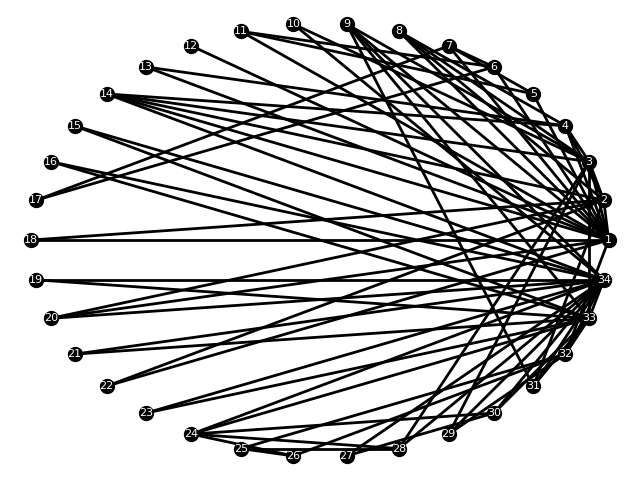
\includegraphics[width=\linewidth]{Figure_1.png}
  \caption{Graph of karate club network.}
  \label{fig:graph model}
\end{figure}

Figure \ref{fig:graph model} shows a graph of the karate club network.

\subsection{}
Zachary\cite{Zachary} analyzes the splintering of a karate club into two different organizations
over a dispute over lessen fees. He lists several reasons for formalizing this fission
process into a mathematical model, the most important perhaps being that the model is
new to anthropology.\\
\\
His analysis shows how the flow of political information predicts the two opposing
factions' increasingly divergent views and strategy ultimately leading to a fission
as information flow between factions becomes increasingly hampered by a bottleneck
of information between them.\\
\\
Beyond just club meetings, shared perceptions on the nature of the club communicated
in the friendship network was unable to become reconciled accross factional boundraries.
An organizational and ideological feedback relationship -- a vicious cycle-- wherein the
strategy of the factions increasingly intensified the ideological divide while threatening
the organizational basis for the network's existence itself made the fission all but
inevitable.\\
\\
The form of this analysis can be applied to more than just the karate club, extending to
analysis of communication patterns in small groups in general due to the inherency of the
the feature of the minimum cut in a capacitated network in this mathematical model, which
is what made this model quite new to anthropology at the time. Whenever the existence of
a unique minimum cut in a capacitated network can be established, it will under certain
conditions (here communication of club meetings) result in a barrier to group unity which
can end up in a group fission.

\subsection{}
Running the following functions yielded the following results:\\
\\
degree\_centrality(G)\\
1: 0.48484848484848486, 2: 0.2727272727272727, 3: 0.30303030303030304,
4: 0.18181818181818182, 5: 0.09090909090909091, 6: 0.12121212121212122,
7: 0.12121212121212122, 8: 0.12121212121212122, 9: 0.15151515151515152,
10: 0.06060606060606061, 11: 0.09090909090909091, 12: 0.030303030303030304,
13: 0.06060606060606061, 14: 0.15151515151515152, 15: 0.06060606060606061,
16: 0.06060606060606061, 17: 0.06060606060606061, 18: 0.06060606060606061,
19: 0.06060606060606061, 20: 0.09090909090909091, 21: 0.06060606060606061,
22: 0.06060606060606061, 23: 0.06060606060606061, 24: 0.15151515151515152,
25: 0.09090909090909091, 26: 0.09090909090909091, 27: 0.06060606060606061,
28: 0.12121212121212122, 29: 0.09090909090909091, 30: 0.12121212121212122,
31: 0.12121212121212122, 32: 0.18181818181818182, 33: 0.36363636363636365,
34: 0.5151515151515151
\\\\
betweenness\_centrality(G)\\
1: 0.43763528138528146, 2: 0.053936688311688304, 3: 0.14365680615680618,
4: 0.011909271284271283, 5: 0.0006313131313131313, 6: 0.02998737373737374,
7: 0.029987373737373736, 8: 0.0, 9: 0.05592682780182781, 10: 0.0008477633477633478,
11: 0.0006313131313131313, 12: 0.0, 13: 0.0, 14: 0.04586339586339586, 15: 0.0,
16: 0.0, 17: 0.0, 18: 0.0, 19: 0.0, 20: 0.03247504810004811, 21: 0.0, 22: 0.0,
23: 0.0, 24: 0.017613636363636363, 25: 0.0022095959595959595, 26: 0.0038404882154882154,
27: 0.0, 28: 0.02233345358345358, 29: 0.0017947330447330447, 30: 0.0029220779220779218,
31: 0.014411976911976909, 32: 0.13827561327561325, 33: 0.145247113997114, 34: 0.30407497594997596
\\\\
closeness\_centrality(G)\\
1: 0.5689655172413793, 2: 0.4852941176470588, 3: 0.559322033898305,
4: 0.4647887323943662, 5: 0.3793103448275862, 6: 0.38372093023255816,
7: 0.38372093023255816, 8: 0.44, 9: 0.515625, 10: 0.4342105263157895,
11: 0.3793103448275862, 12: 0.36666666666666664, 13: 0.3707865168539326,
14: 0.515625, 15: 0.3707865168539326, 16: 0.3707865168539326, 17: 0.28448275862068967,
18: 0.375, 19: 0.3707865168539326, 20: 0.5, 21: 0.3707865168539326,
22: 0.375, 23: 0.3707865168539326, 24: 0.39285714285714285, 25: 0.375,
26: 0.375, 27: 0.3626373626373626, 28: 0.4583333333333333, 29: 0.4520547945205479,
30: 0.38372093023255816, 31: 0.4583333333333333, 32: 0.5409836065573771, 33: 0.515625, 34: 0.55
\\\\
average\_clustering(G)\\
0.5706384782076823
\\\\
connectivity.local\_edge\_connectivity(G, 1, 34)\\
10

\section{Polarized blogging about climate change}
\subsection{}
Statistics:\\
Average degree: \hfill 2.524\\
Network diameter: \hfill 4\\
Graph density (undirected): \hfill 0.001\\
Modularity: \hfill 0.667\\
Connected components: \hfill 1\\
Average Clustering Coefficient: \hfill 0.249\\
Average path length: \hfill 3.236\\
\\
\begin{figure}
  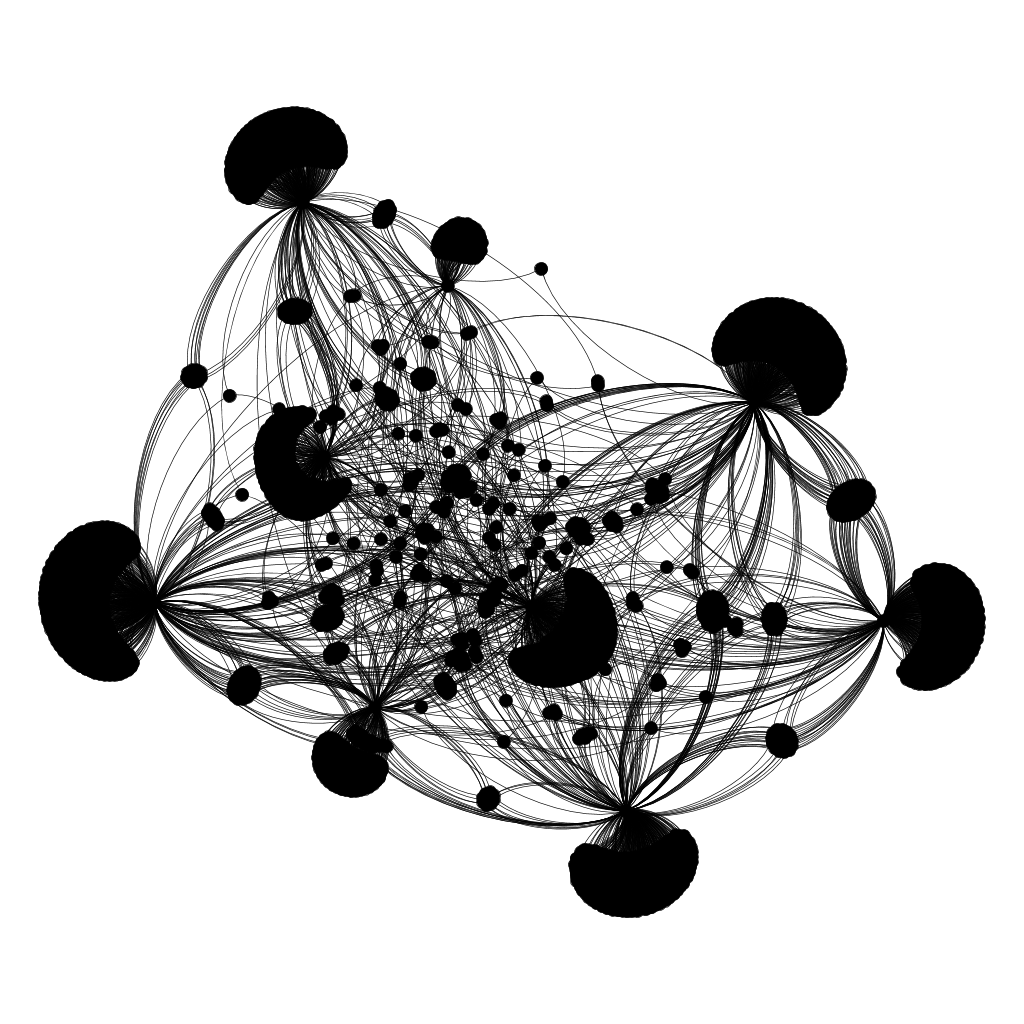
\includegraphics[width=\linewidth]{Figure_2.png}
  \caption{A graph of the network.}
  \label{fig:graph}
\end{figure}

Figure \ref{fig:graph} shows a graph of the network of climate blogs.

\subsection{}
\textbf{https://wattsupwiththat.com/}\\
Anthony is a former meteorologist who appears to express his position on climate
change emotively by cataloging percieved faults by those who adhere to the fact of
anthropogenic global warming in what he calles ''Climate FAIL Files''. Interestingly
he lists the following as the reason for changing his mind about climate change on
the FAQ page:

\begin{displayquote}
\textit{My questioning started due to a professional friendship that came
about with Jim Goodridge. [...] He had showed me some of his investigations into
California’s temperature and precipitation records that didn’t quite add up to some
of the claims about warming I was reading about.}
\end{displayquote}

\textbf{https://www.desmogblog.com}\\
The position on climate change in this blog appears to be staunchly against
the views expressed by climate deniers, aiming to catalog all disinformation
campaigns in the ''Climate Disinformation Database''. As it says on the
database page:

\begin{displayquote}
\textit{DeSmogBlog thoroughly investigates the academic and industry backgrounds of those
involved in the PR spin campaigns that are confusing the public and stalling action
on global warming.}
\end{displayquote}

\textbf{http://joannenova.com.au/}\\
Jo expresses her views on climate change by insinuating that scientists working on
data which confirms the reality of global warming are motivated by money and that
their data doesn't stand up to scrutiny due to things like spelling errors,
ostensible elementary mistakes in the data itself, and lack of audit and control
despite papers having to be submitted to a rigorous peer review process.\\
\\
\textbf{https://judithcurry.com/}\\
Judith's blog presents itself on the about page as follows:

\begin{displayquote}
\textit{Climate Etc. provides a forum for climate researchers, academics and technical experts
from other fields, citizen scientists, and the interested public to engage in a
discussion on topics related to climate science and the science-policy interface.}
\end{displayquote}

There doesn't appear to be any ideological position taken and the blog's purpose
is to encourage debate around climate science.\\
\\
\textbf{http://www.climatecentral.org/}\\
Climate Central presents themselves as follows:

\begin{displayquote}
\textit{An independent organization of leading scientists and journalists researching and
reporting the facts about our changing climate and its impact on the public.}
\end{displayquote}

They express their views on climate change as it being a reality, presents its
effects, backs it up with research and data, and discusses possible solutions to the
problem as well as what's being done and has been done so far.\\

\textbf{https://insideclimatenews.org/}\\
ICN accept the reality of climate change and seeks to act as watchdog against
governments and groups that pose a threat to the vital work needed to combat it.
They cover all news related to climate change including policies that affect it.
As it reads on their about page:

\begin{displayquote}
\textit{InsideClimate News is an independent, not-for-profit, non-partisan news organization
that covers clean energy, carbon energy, nuclear energy and environmental science—plus
the territory in between where law, policy and public opinion are shaped.}
\end{displayquote}

\textbf{http://www.climatechangenews.com/}\\
Very much the same as the former:

\begin{displayquote}
\textit{Climate Home News is an independent news site dedicated to bringing important climate
stories to as large an audience as possible.}
\end{displayquote}


\textbf{http://www.realclimate.org/}\\
RealClimate presents news about climate change in the eyes of climate scientists. It
allows comments on its posts which encourages discussion around the science of
climate change for anyone interested. Unsurprisingly they do not deny the reality of
anthropogenic global warming.  As it reads on their about page:

\begin{displayquote}
\textit{RealClimate is a commentary site on climate science by working climate scientists for
the interested public and journalists. We aim to provide a quick response to developing
stories and provide the context sometimes missing in mainstream commentary. The
discussion here is mostly restricted to scientific topics and will only rarely get
involved in any political or economic implications of the science.}
\end{displayquote}


\textbf{https://www.skepticalscience.com/}\\
SkepticalScience combats the misinformation by climate deniers by debunking their
claims head on and looking at what the evidence actually says. It was created by
John Cook, a cognitive scientist. As it reads on the front page:

\begin{displayquote}
\textit{Scientific skepticism is healthy. Scientists should always challenge themselves to
improve their understanding. Yet this isn't what happens with climate change denial.
Skeptics vigorously criticise any evidence that supports man-made global warming and
yet embrace any argument, op-ed, blog or study that purports to refute global warming.
This website gets skeptical about global warming skepticism. Do their arguments have
any scientific basis? What does the peer reviewed scientific literature say?}
\end{displayquote}

\section{The psychology of social media}


\pagebreak
\bibliography{references.bib}
\bibliographystyle{ieeetr}

\end{document}
